\usetikzlibrary{arrows.meta,shapes.multipart}
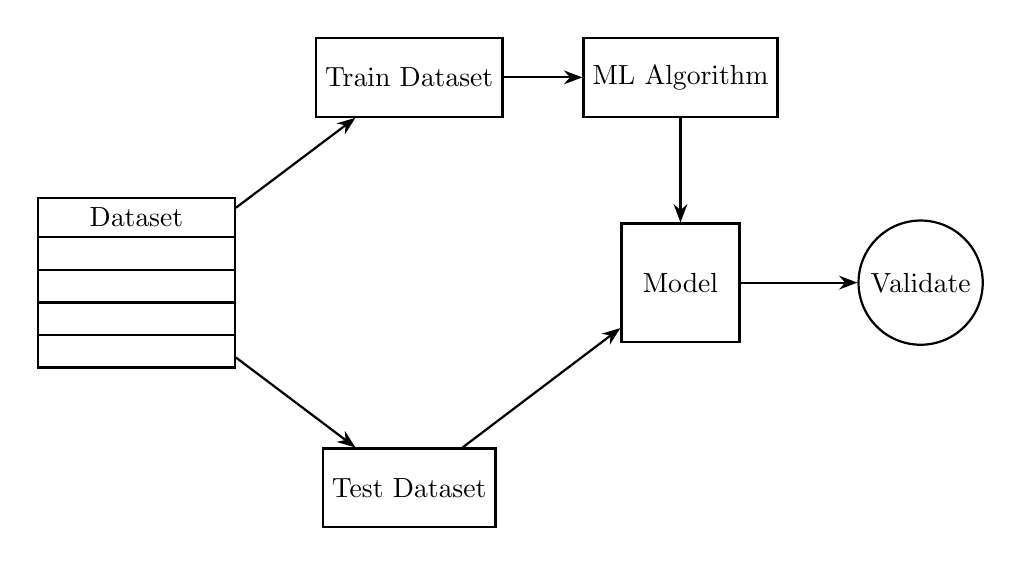
\begin{tikzpicture}[
  thick,>={Stealth[]},
  ampersand replacement=\&,
  circ/.style = {draw,circle,minimum size=1cm},
  rect/.style = {draw,rectangle,minimum size=1cm},
  splt/.style = {draw,rectangle split,rectangle split parts=5,minimum size=0.5cm}
  ]
  \matrix[row sep=1cm,column sep=1cm] {
     {}; \&
     \node[rect] (Tr) {Train Dataset};  \&
     \node[rect] (A) {ML Algorithm}; \&
     {};\\

     \node[splt, minimum size=25mm] (D) {Dataset}; \&
     {};\&
     \node[rect, minimum size=15mm] (M) {Model}; \&
     \node[circ] (V) {Validate};\\

     {};\&
     \node[rect] (Te) {Test Dataset};
     {}; \&
     {}; \&\\
  };
  \draw[->] (D)  --(Tr);
  \draw[->] (D) --(Te);
  \draw[->] (Tr) --(A);
  \draw[->] (Te) --(M);
  \draw[->] (A) --(M);
  \draw[->] (M) --(V);
\end{tikzpicture}
